\clearpage
\SourceLeaf{002}\pdfbookmark[0]{Works. Volume VII}{werke-cover}
\thispagestyle{empty}
\begin{center}
\vspace*{.8in}
{\Large CARL FRIEDRICH GAUSS}\par\bigskip
{\Huge WORKS}\par\bigskip
{\large VOLUME VII}\par\vspace{.6in}
EDITED\par\medskip
BY THE\par\bigskip
{\small ROYAL SOCIETY OF SCIENCES}\par\medskip
AT\par\bigskip
{\large GÖTTINGEN}\par\vfill
{\small DISTRIBUTED BY B. G. TEUBNER IN LEIPZIG}\par\medskip
1906.
\end{center}
\clearpage
\SourceLeaf{004}\pdfbookmark[1]{Works. Volume VII. (Half Title)}{half-title}
\thispagestyle{empty}
\begin{center}\vspace*{2.3in}
{\Large THE WORKS OF CARL FRIEDRICH GAUSS}\par\bigskip
{\large VOLUME VII.}
\end{center}
\clearpage
\SourceLeaf{006}\pdfbookmark[1]{Works. Volume VII. (Illustrated Title Page)}{werke-title}
\thispagestyle{empty}
\begin{center}
{\Large CARL FRIEDRICH GAUSS}\par\bigskip
{\Huge WORKS}\par\bigskip
{\large VOLUME VII.}\par\medskip
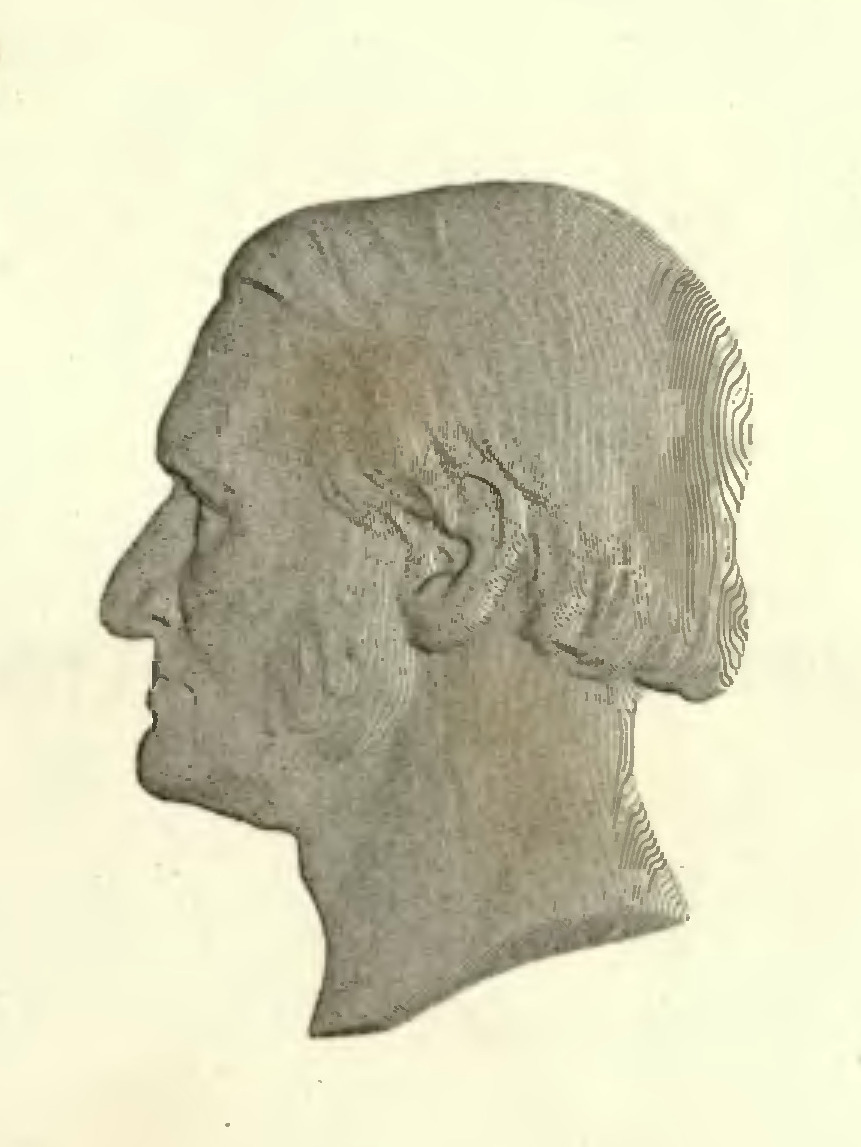
\includegraphics[height=2.05in]{images/gauss_title_vignette_1870.jpg}\par\medskip
EDITED\par\smallskip
BY THE\par\medskip
{\small ROYAL SOCIETY OF SCIENCES}\par\smallskip
AT\par\medskip
{\large GÖTTINGEN.}\par\vfill
{\small DISTRIBUTED BY B. G. TEUBNER IN LEIPZIG.}\par\medskip
1906.
\end{center}
\clearpage
\SourceLeaf{008}\pdfbookmark[0]{Theory of the Motion of Celestial Bodies}{theoria-title}
\thispagestyle{empty}
\begin{center}
\vspace*{.3in}
{\LARGE THEORY}\par\bigskip
{\Large OF THE MOTION}\par\bigskip
{\Large OF CELESTIAL BODIES}\par\bigskip
IN\par\bigskip
{\small CONIC SECTIONS AROUND THE SUN}\par\bigskip
BY\par\bigskip
{\large CARL FRIEDRICH GAUSS}\par\bigskip
\rule{.6\linewidth}{.3pt}\par\bigskip
{\small PUBLISHED IN HAMBURG BY FRID. PERTHES AND I. H. BESSER}\par\medskip
1809.\par\medskip
\rule{.3\linewidth}{.3pt}\par\bigskip
Sold by
\end{center}
{\footnotesize\noindent
\begin{tabular*}{\linewidth}{@{}l@{\extracolsep{\fill}}l@{}}
\textsc{Paris,} Treuttel \& Würtz. & \textsc{London,} R. H. Evans.\\
\textsc{Stockholm,} A. Wiborg. & \textsc{St Petersburg,} Klostermann.\\
\textsc{Madrid,} Sancha. & \textsc{Florence,} Molini, Landi \& C\raisebox{.2ex}{\scriptsize o}.\\
\end{tabular*}\par\smallskip\noindent
\textsc{Amsterdam,} at the bookshop called Kunst- und Industrie-Comptoir.\par}
